% Options for packages loaded elsewhere
\PassOptionsToPackage{unicode}{hyperref}
\PassOptionsToPackage{hyphens}{url}
%
\documentclass[
]{article}
\usepackage{amsmath,amssymb}
\usepackage{iftex}
\ifPDFTeX
  \usepackage[T1]{fontenc}
  \usepackage[utf8]{inputenc}
  \usepackage{textcomp} % provide euro and other symbols
\else % if luatex or xetex
  \usepackage{unicode-math} % this also loads fontspec
  \defaultfontfeatures{Scale=MatchLowercase}
  \defaultfontfeatures[\rmfamily]{Ligatures=TeX,Scale=1}
\fi
\usepackage{lmodern}
\ifPDFTeX\else
  % xetex/luatex font selection
\fi
% Use upquote if available, for straight quotes in verbatim environments
\IfFileExists{upquote.sty}{\usepackage{upquote}}{}
\IfFileExists{microtype.sty}{% use microtype if available
  \usepackage[]{microtype}
  \UseMicrotypeSet[protrusion]{basicmath} % disable protrusion for tt fonts
}{}
\makeatletter
\@ifundefined{KOMAClassName}{% if non-KOMA class
  \IfFileExists{parskip.sty}{%
    \usepackage{parskip}
  }{% else
    \setlength{\parindent}{0pt}
    \setlength{\parskip}{6pt plus 2pt minus 1pt}}
}{% if KOMA class
  \KOMAoptions{parskip=half}}
\makeatother
\usepackage{xcolor}
\usepackage[margin=1in]{geometry}
\usepackage{graphicx}
\makeatletter
\newsavebox\pandoc@box
\newcommand*\pandocbounded[1]{% scales image to fit in text height/width
  \sbox\pandoc@box{#1}%
  \Gscale@div\@tempa{\textheight}{\dimexpr\ht\pandoc@box+\dp\pandoc@box\relax}%
  \Gscale@div\@tempb{\linewidth}{\wd\pandoc@box}%
  \ifdim\@tempb\p@<\@tempa\p@\let\@tempa\@tempb\fi% select the smaller of both
  \ifdim\@tempa\p@<\p@\scalebox{\@tempa}{\usebox\pandoc@box}%
  \else\usebox{\pandoc@box}%
  \fi%
}
% Set default figure placement to htbp
\def\fps@figure{htbp}
\makeatother
\setlength{\emergencystretch}{3em} % prevent overfull lines
\providecommand{\tightlist}{%
  \setlength{\itemsep}{0pt}\setlength{\parskip}{0pt}}
\setcounter{secnumdepth}{-\maxdimen} % remove section numbering
\ifLuaTeX
\usepackage[bidi=basic]{babel}
\else
\usepackage[bidi=default]{babel}
\fi
\babelprovide[main,import]{french}
% get rid of language-specific shorthands (see #6817):
\let\LanguageShortHands\languageshorthands
\def\languageshorthands#1{}
\usepackage{bookmark}
\IfFileExists{xurl.sty}{\usepackage{xurl}}{} % add URL line breaks if available
\urlstyle{same}
\hypersetup{
  pdftitle={Enquêtes de conjoncture auprès des entreprises},
  pdfauthor={@statjunior},
  pdflang={fr-FR},
  hidelinks,
  pdfcreator={LaTeX via pandoc}}

\title{Enquêtes de conjoncture auprès des entreprises}
\usepackage{etoolbox}
\makeatletter
\providecommand{\subtitle}[1]{% add subtitle to \maketitle
  \apptocmd{\@title}{\par {\large #1 \par}}{}{}
}
\makeatother
\subtitle{Résultats du mois de juin 2024}
\author{@statjunior}
\date{25 juillet 2024}

\begin{document}
\maketitle

\section{Présentation}\label{pruxe9sentation}

Ce rapport \emph{RMarkdown} présente les résultats des enquêtes de
conjoncture auprès des entreprises réalisées par l'Insee. Le dernier
point connu est juillet 2024.

On présente tout d'abord l'indicateur synthétique du climat des affaires
ainsi que celui de l'emploi pour tous les secteurs de l'économie. Cet
indicateur est de moyenne 100 sur longue période (et d'écart-type 10).

On s'intéresse ensuite au climat des affaires par secteur d'activité
(bâtiment, industrie manufacturière, commerce de détail, services). On
présente également les évolutions de prix et d'emploi prévues par les
chefs d'entreprise de chaque secteur, à un horizon de court-terme.

Enfin, on analyse plus spécifiquement les difficultés de production
présentes dans l'industrie manufacturière, en distinguant les
contraintes d'offre des contraintes de demande.

Ce rapport a été compilé automatiquement avec le logiciel \texttt{R}, le
25 juillet 2024 à 08 heures et 54 minutes. Les potentielles erreurs
présentes dans ce document relèvent uniquement de la responsabilité de
Statjunior.

Le code source permettant de générer ce document est disponible sur Git
\href{https://github.com/statjunior/Statjunior/tree/main/Enqu\%C3\%AAtes\%20de\%20conjoncture/}{en
cliquant ici}.

\section{Climat conjoncturel global}\label{climat-conjoncturel-global}

\subsection{Climat des affaires et de
l'emploi}\label{climat-des-affaires-et-de-lemploi}

\pandocbounded{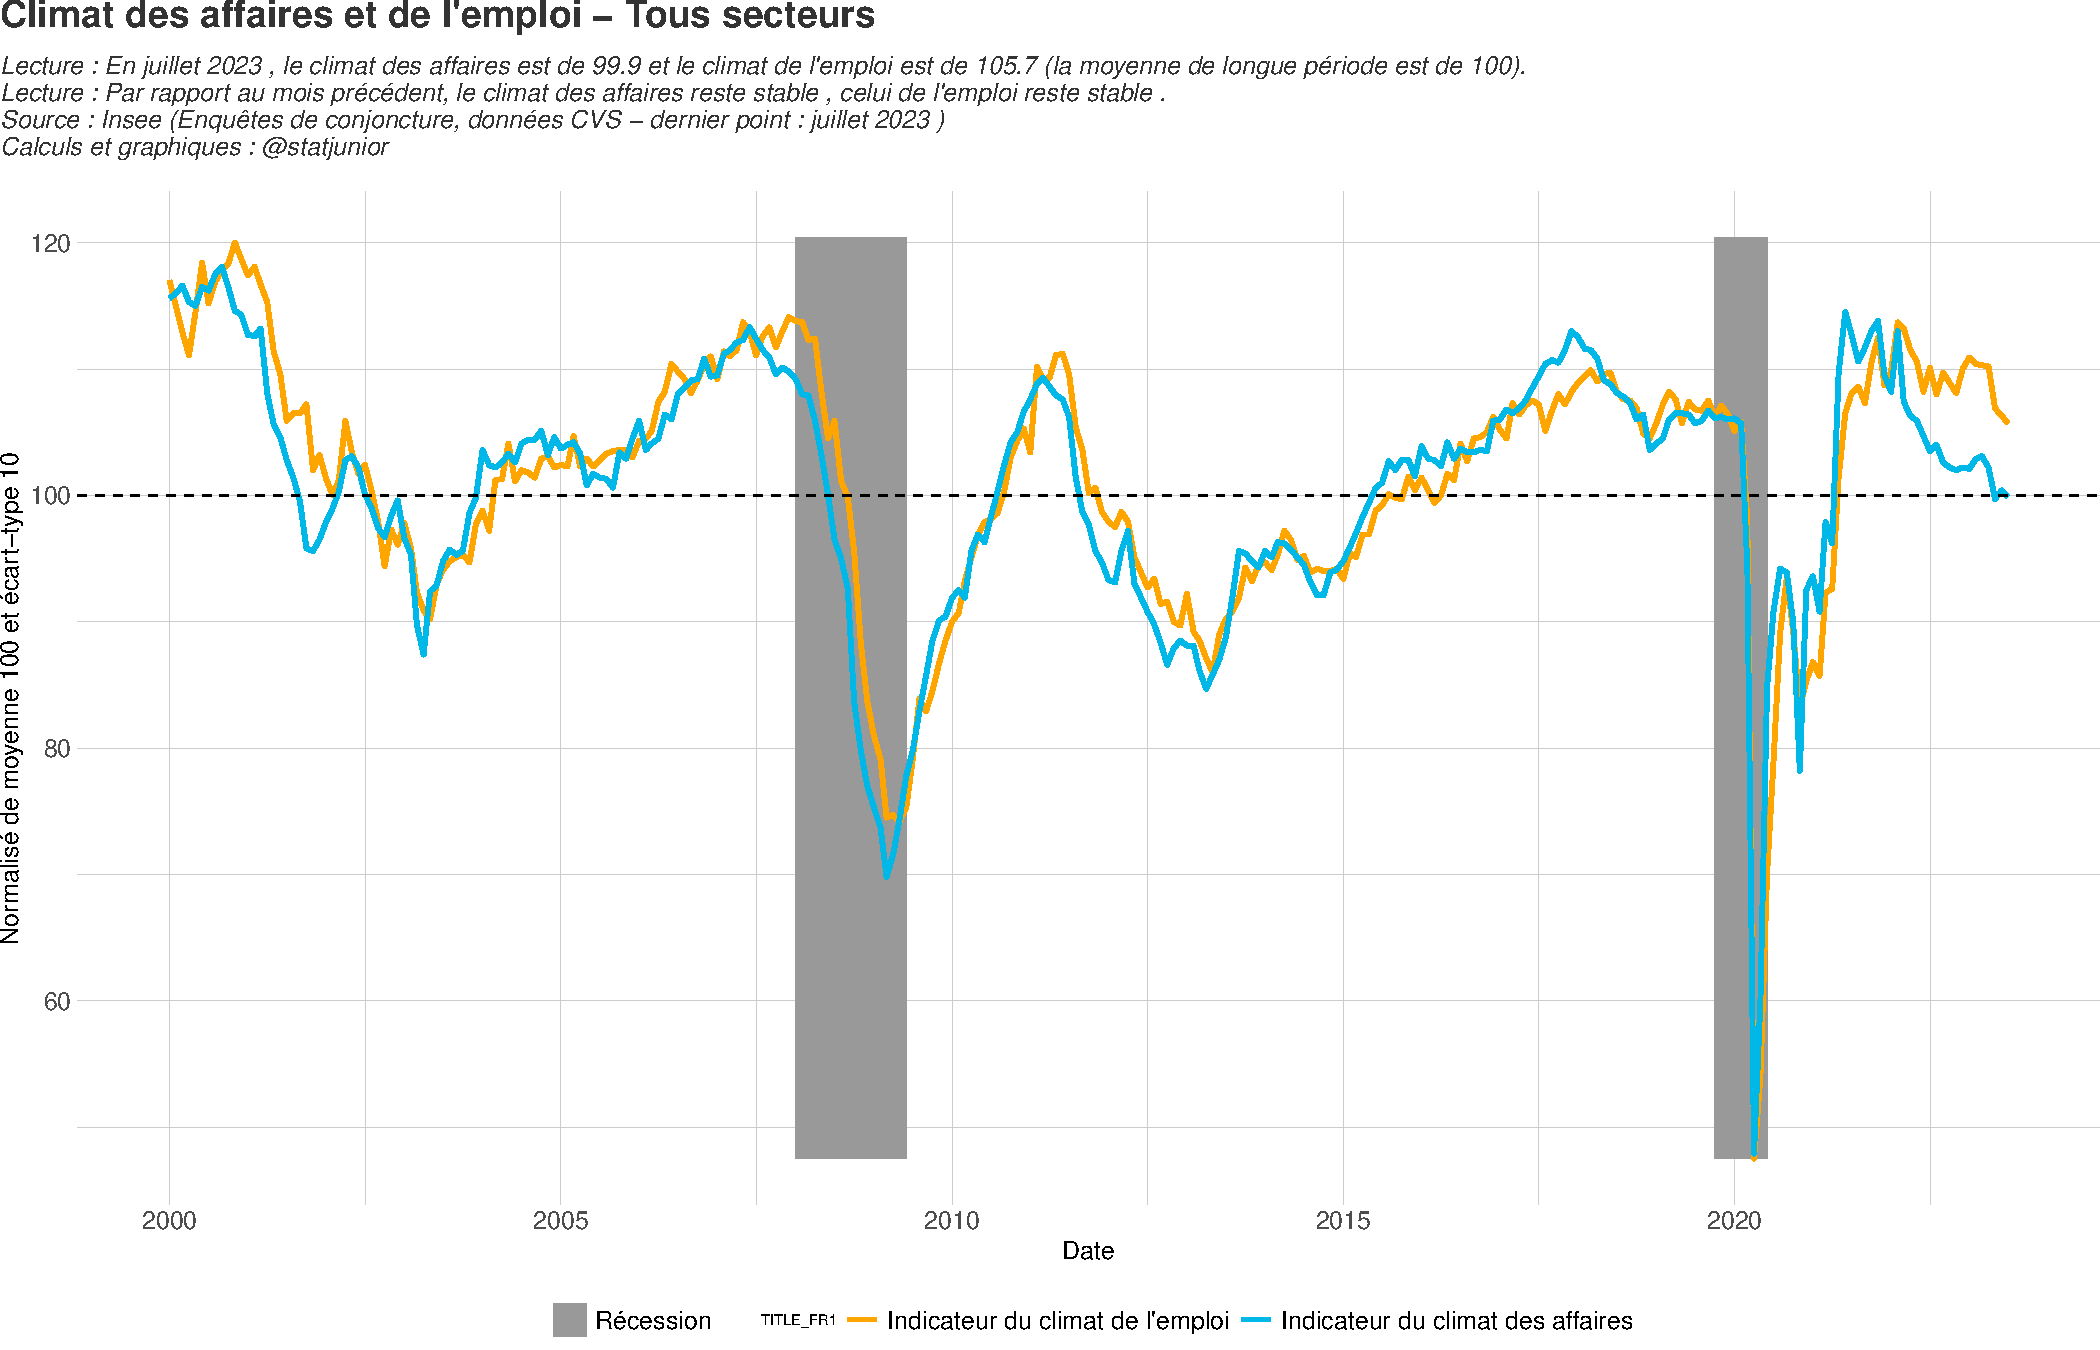
\includegraphics[keepaspectratio]{rapport_pdf_enquete_conj_files/figure-latex/unnamed-chunk-2-1.pdf}}

\subsection{Indicateur de retournement
conjoncturel}\label{indicateur-de-retournement-conjoncturel}

\pandocbounded{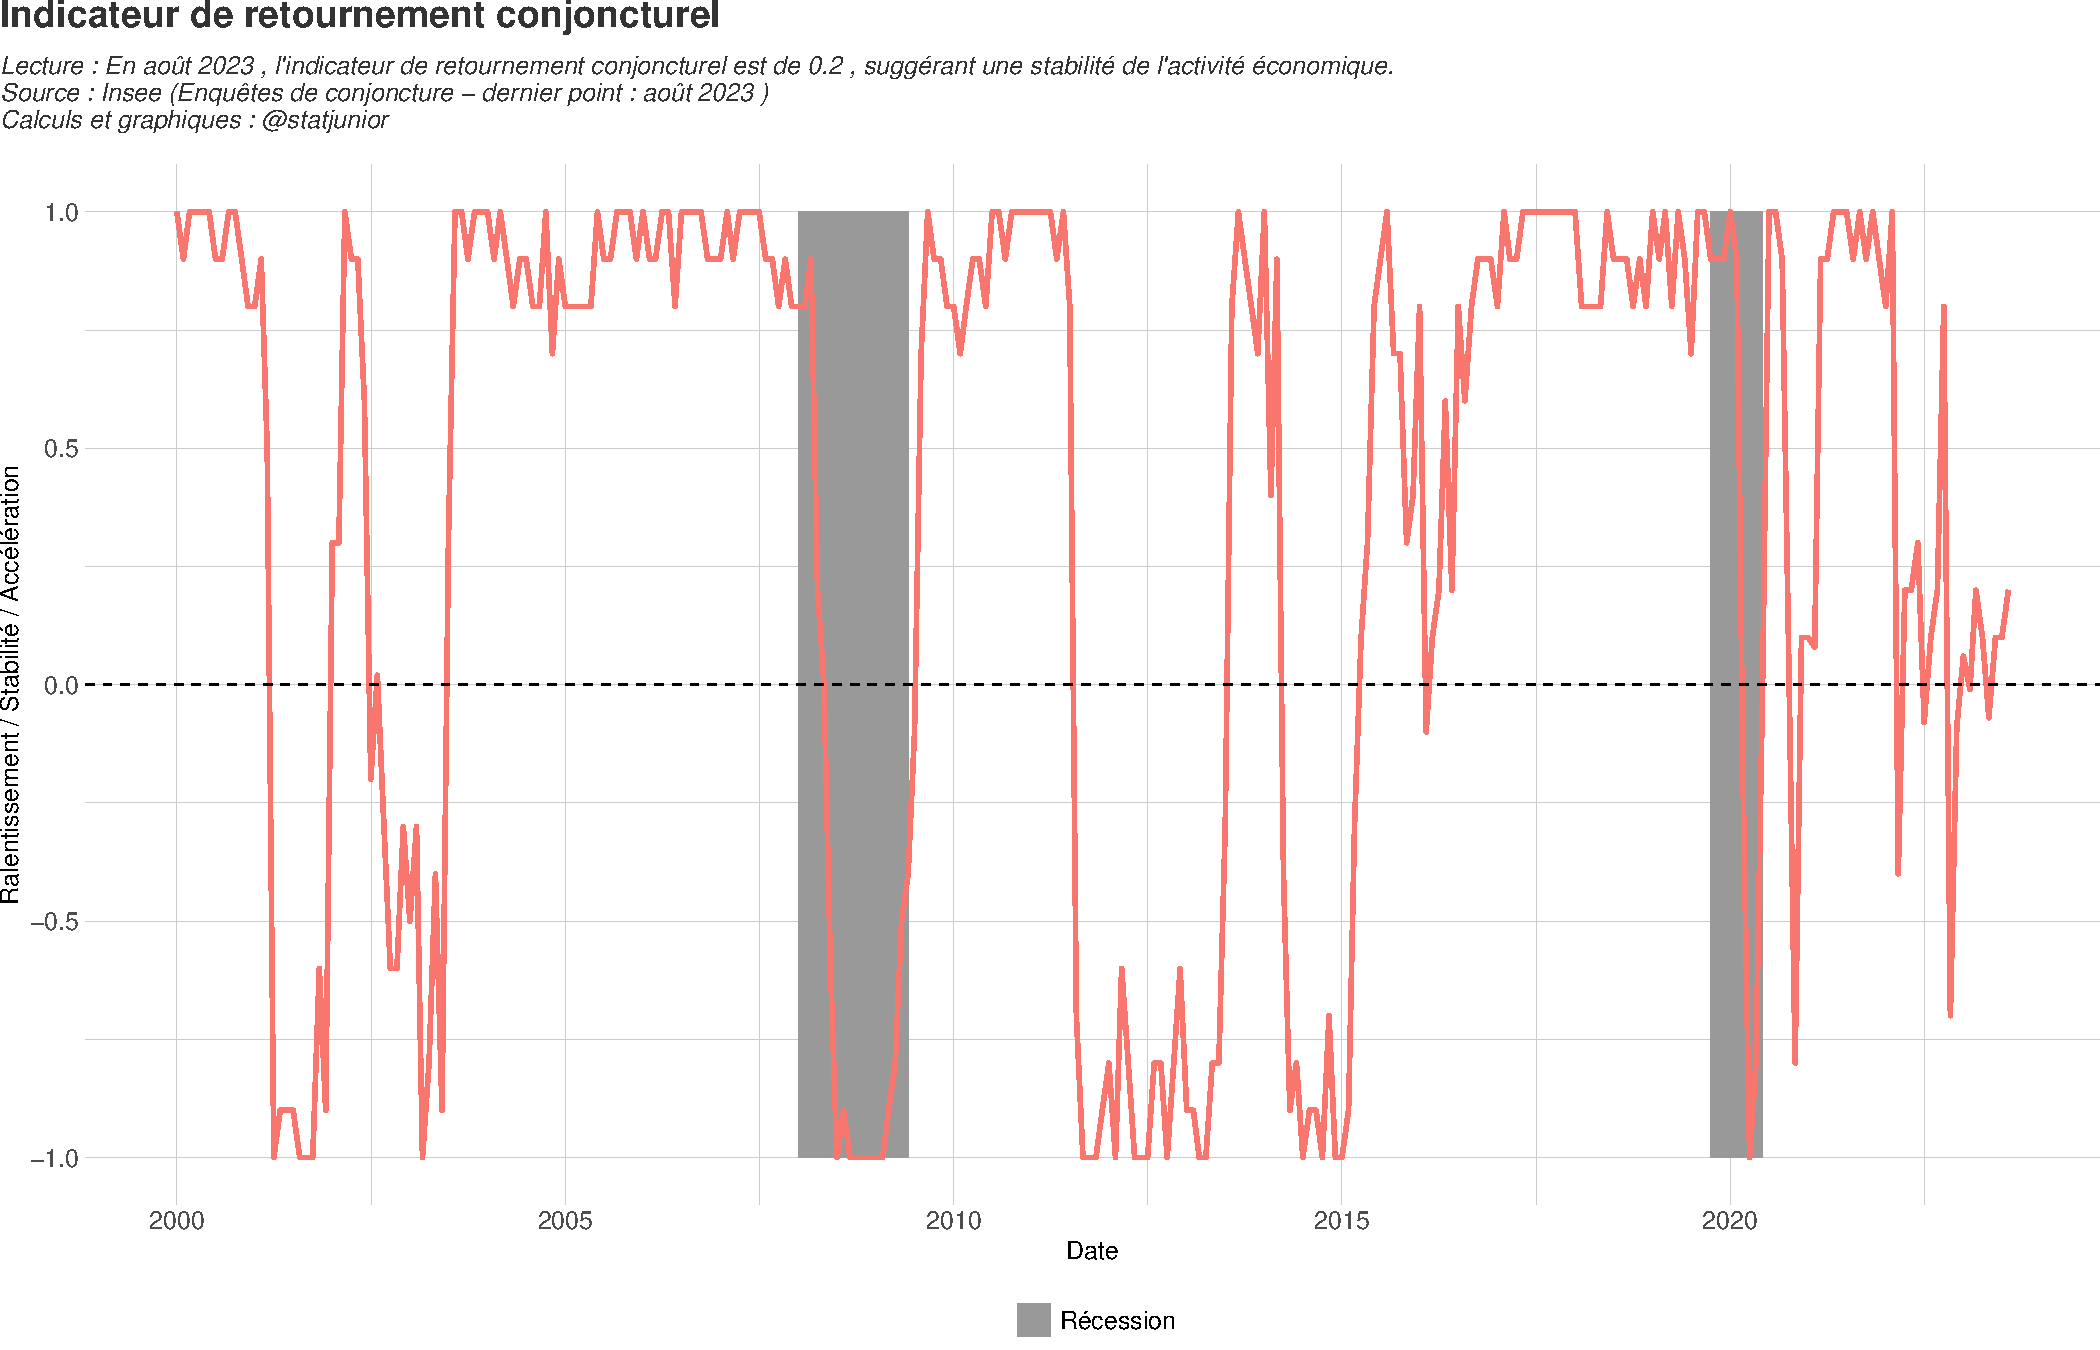
\includegraphics[keepaspectratio]{rapport_pdf_enquete_conj_files/figure-latex/unnamed-chunk-3-1.pdf}}

\section{Climat conjoncturel
sectoriel}\label{climat-conjoncturel-sectoriel}

\subsection{Climat des affaires par
secteur}\label{climat-des-affaires-par-secteur}

\pandocbounded{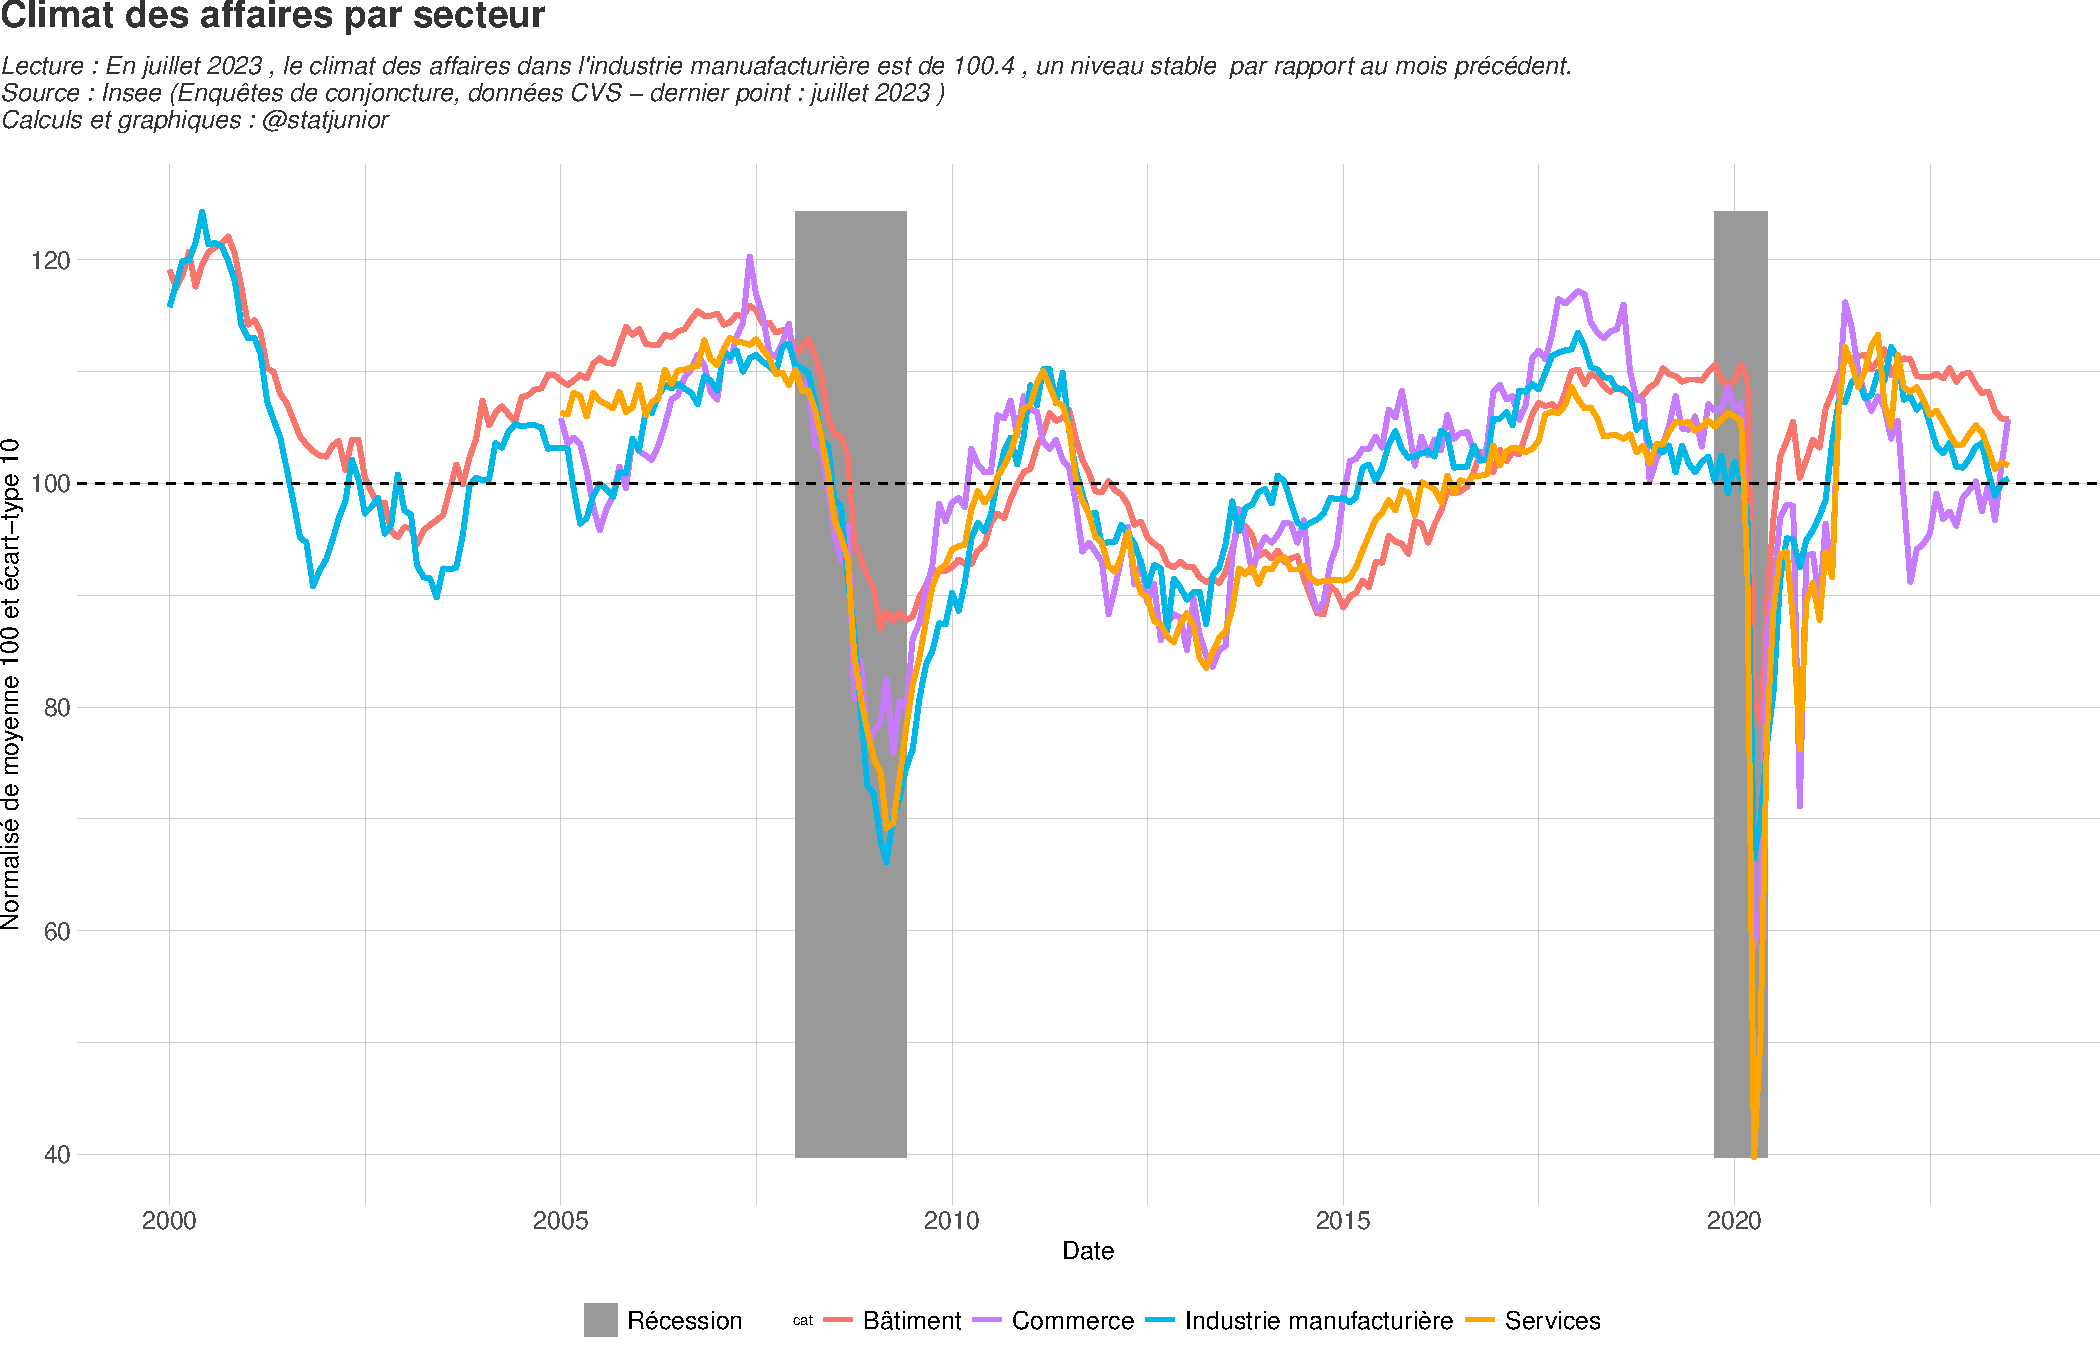
\includegraphics[keepaspectratio]{rapport_pdf_enquete_conj_files/figure-latex/unnamed-chunk-5-1.pdf}}

\subsection{Evolution des prix prévue par
secteur}\label{evolution-des-prix-pruxe9vue-par-secteur}

\pandocbounded{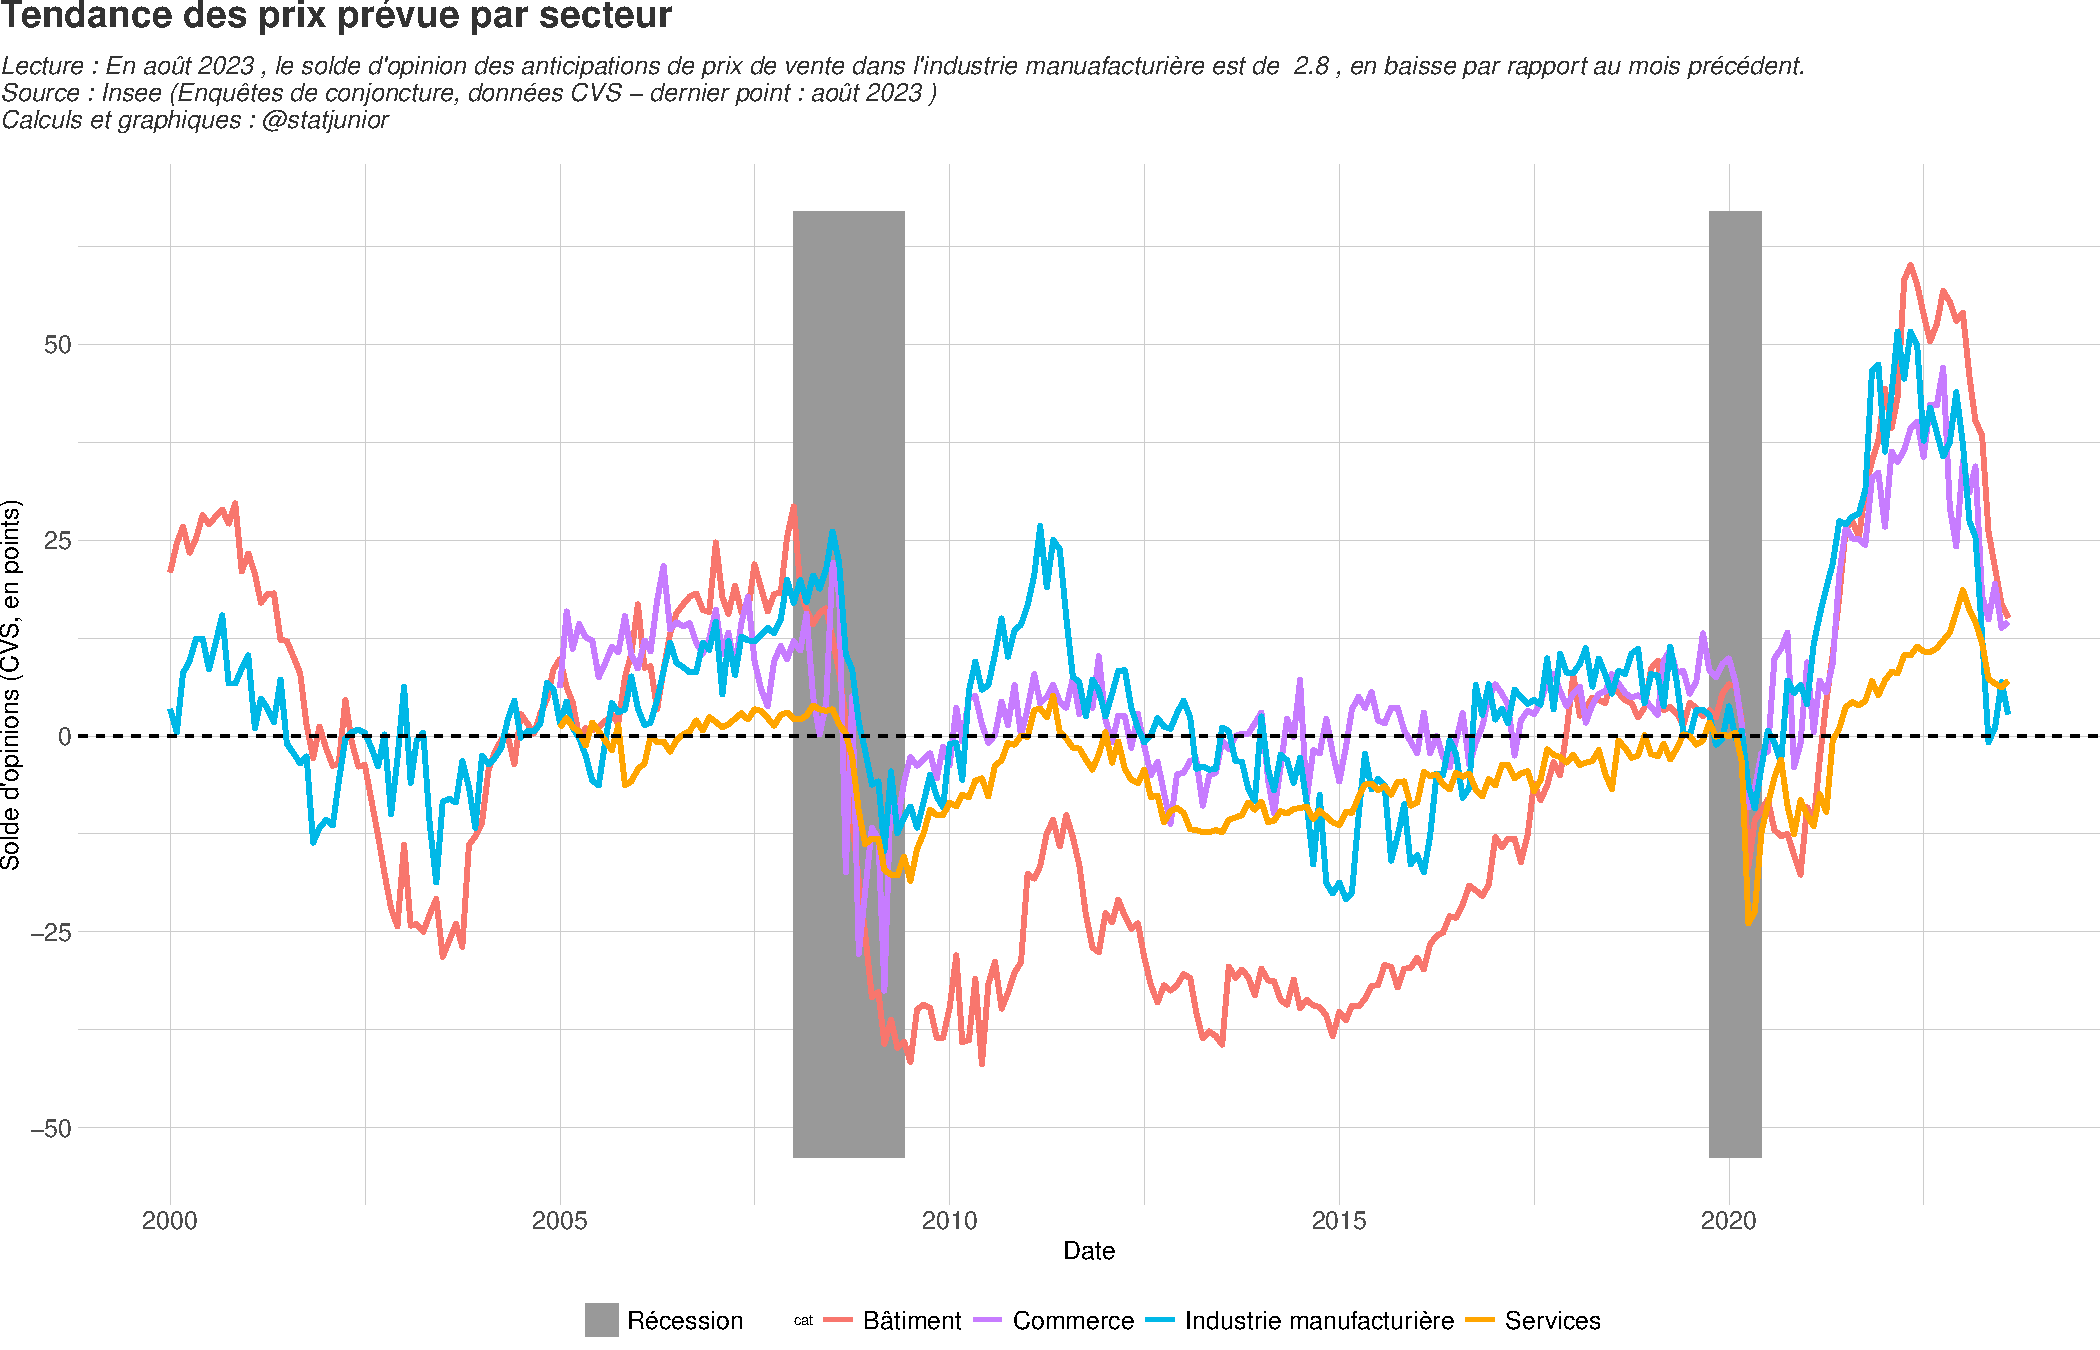
\includegraphics[keepaspectratio]{rapport_pdf_enquete_conj_files/figure-latex/unnamed-chunk-6-1.pdf}}

\subsection{Evolution de l'emploi prévue par
secteur}\label{evolution-de-lemploi-pruxe9vue-par-secteur}

\pandocbounded{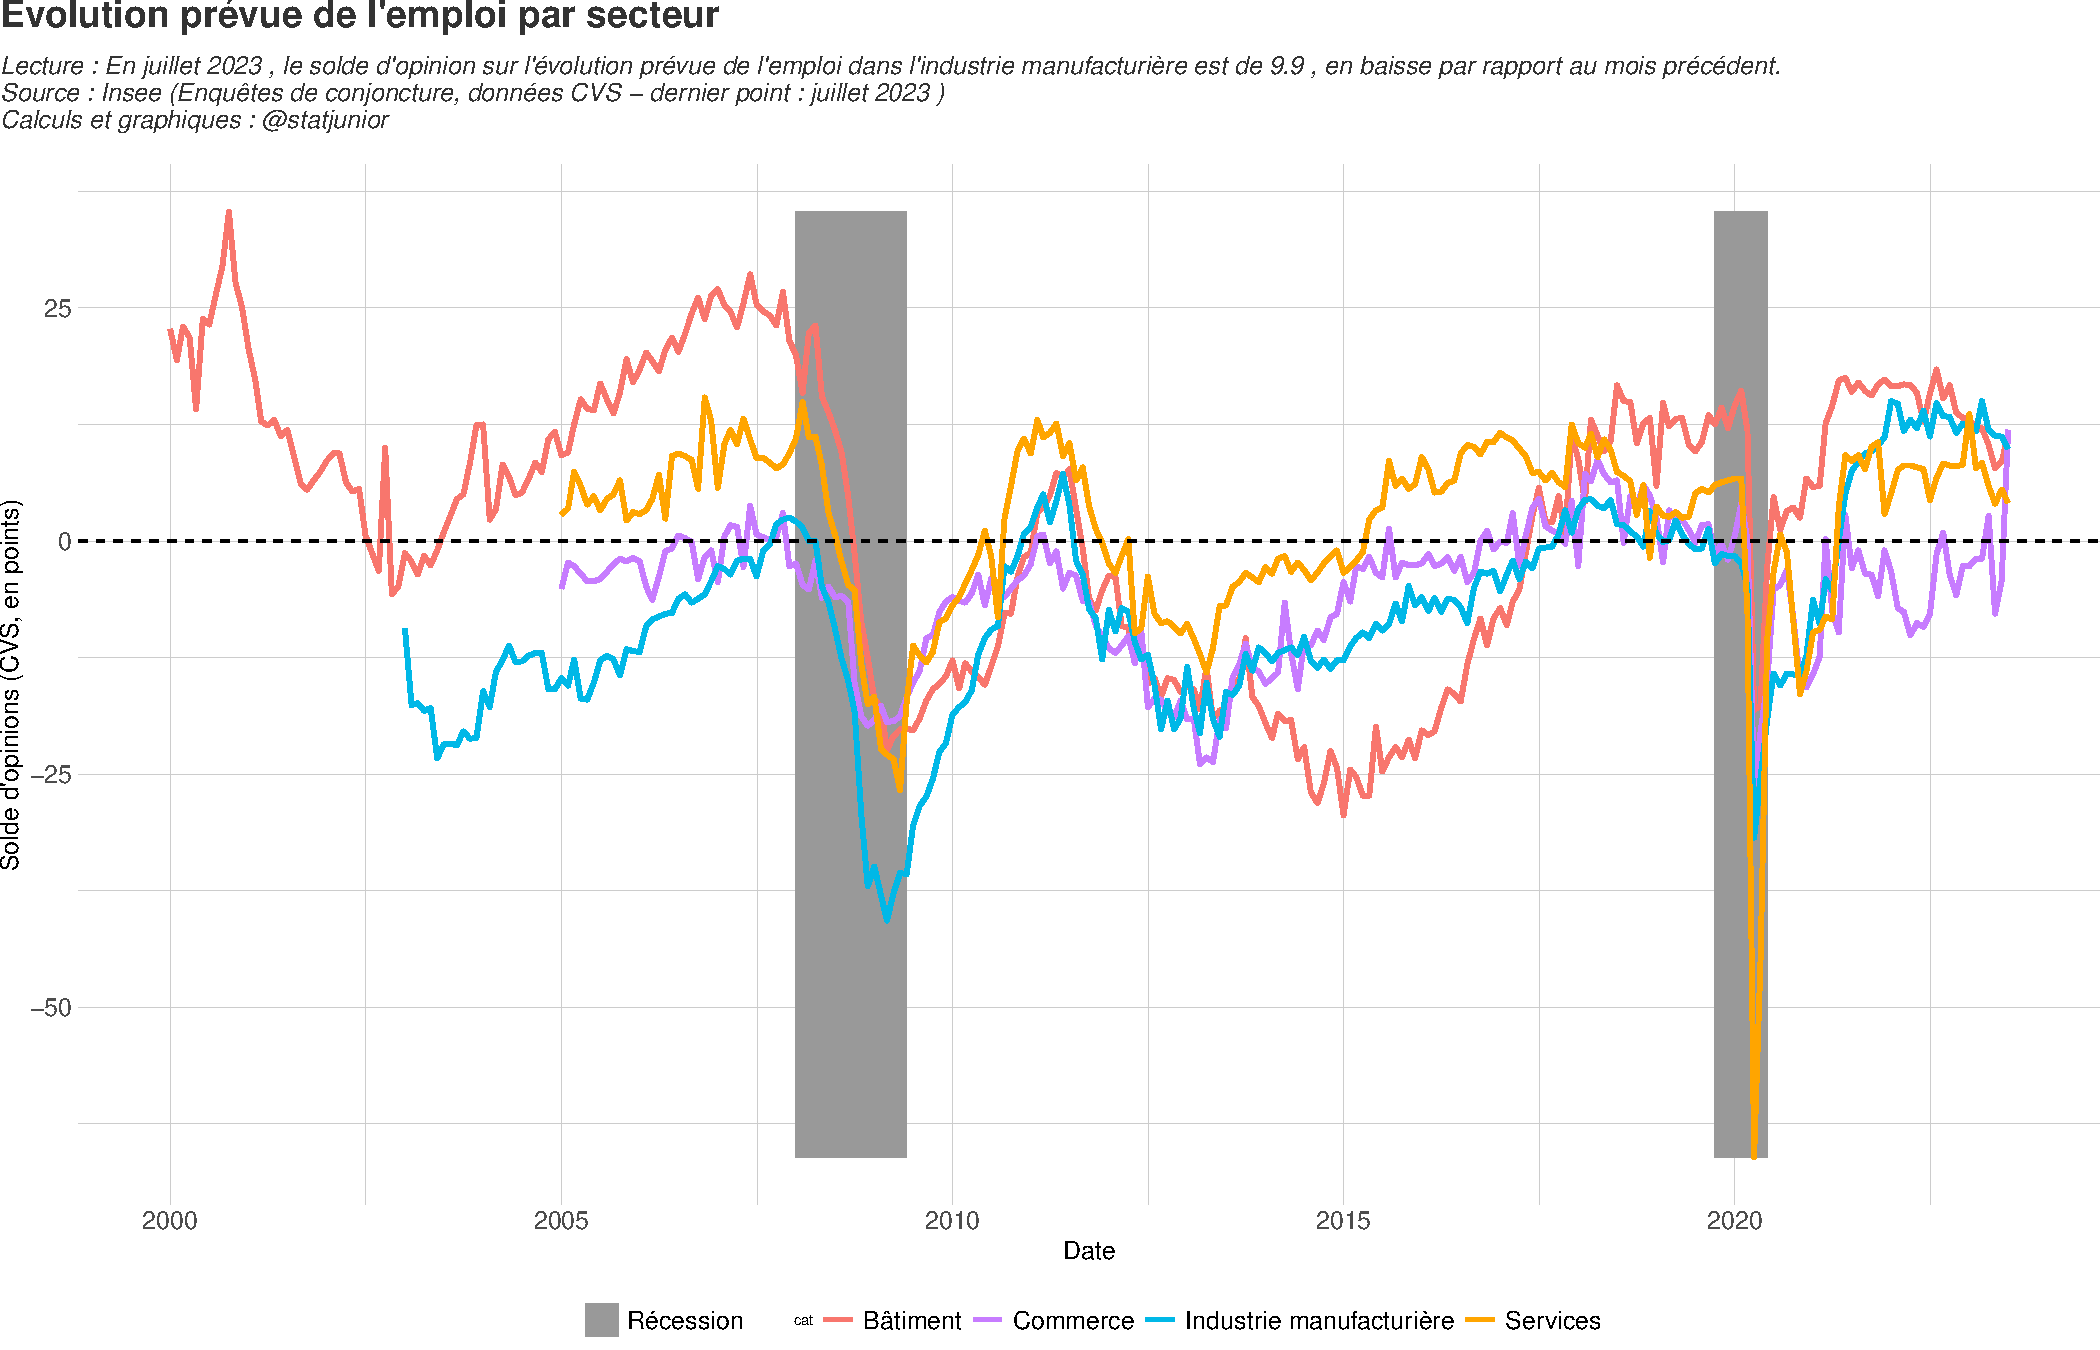
\includegraphics[keepaspectratio]{rapport_pdf_enquete_conj_files/figure-latex/unnamed-chunk-7-1.pdf}}

\section{Contraintes de production dans
l'industrie}\label{contraintes-de-production-dans-lindustrie}

\pandocbounded{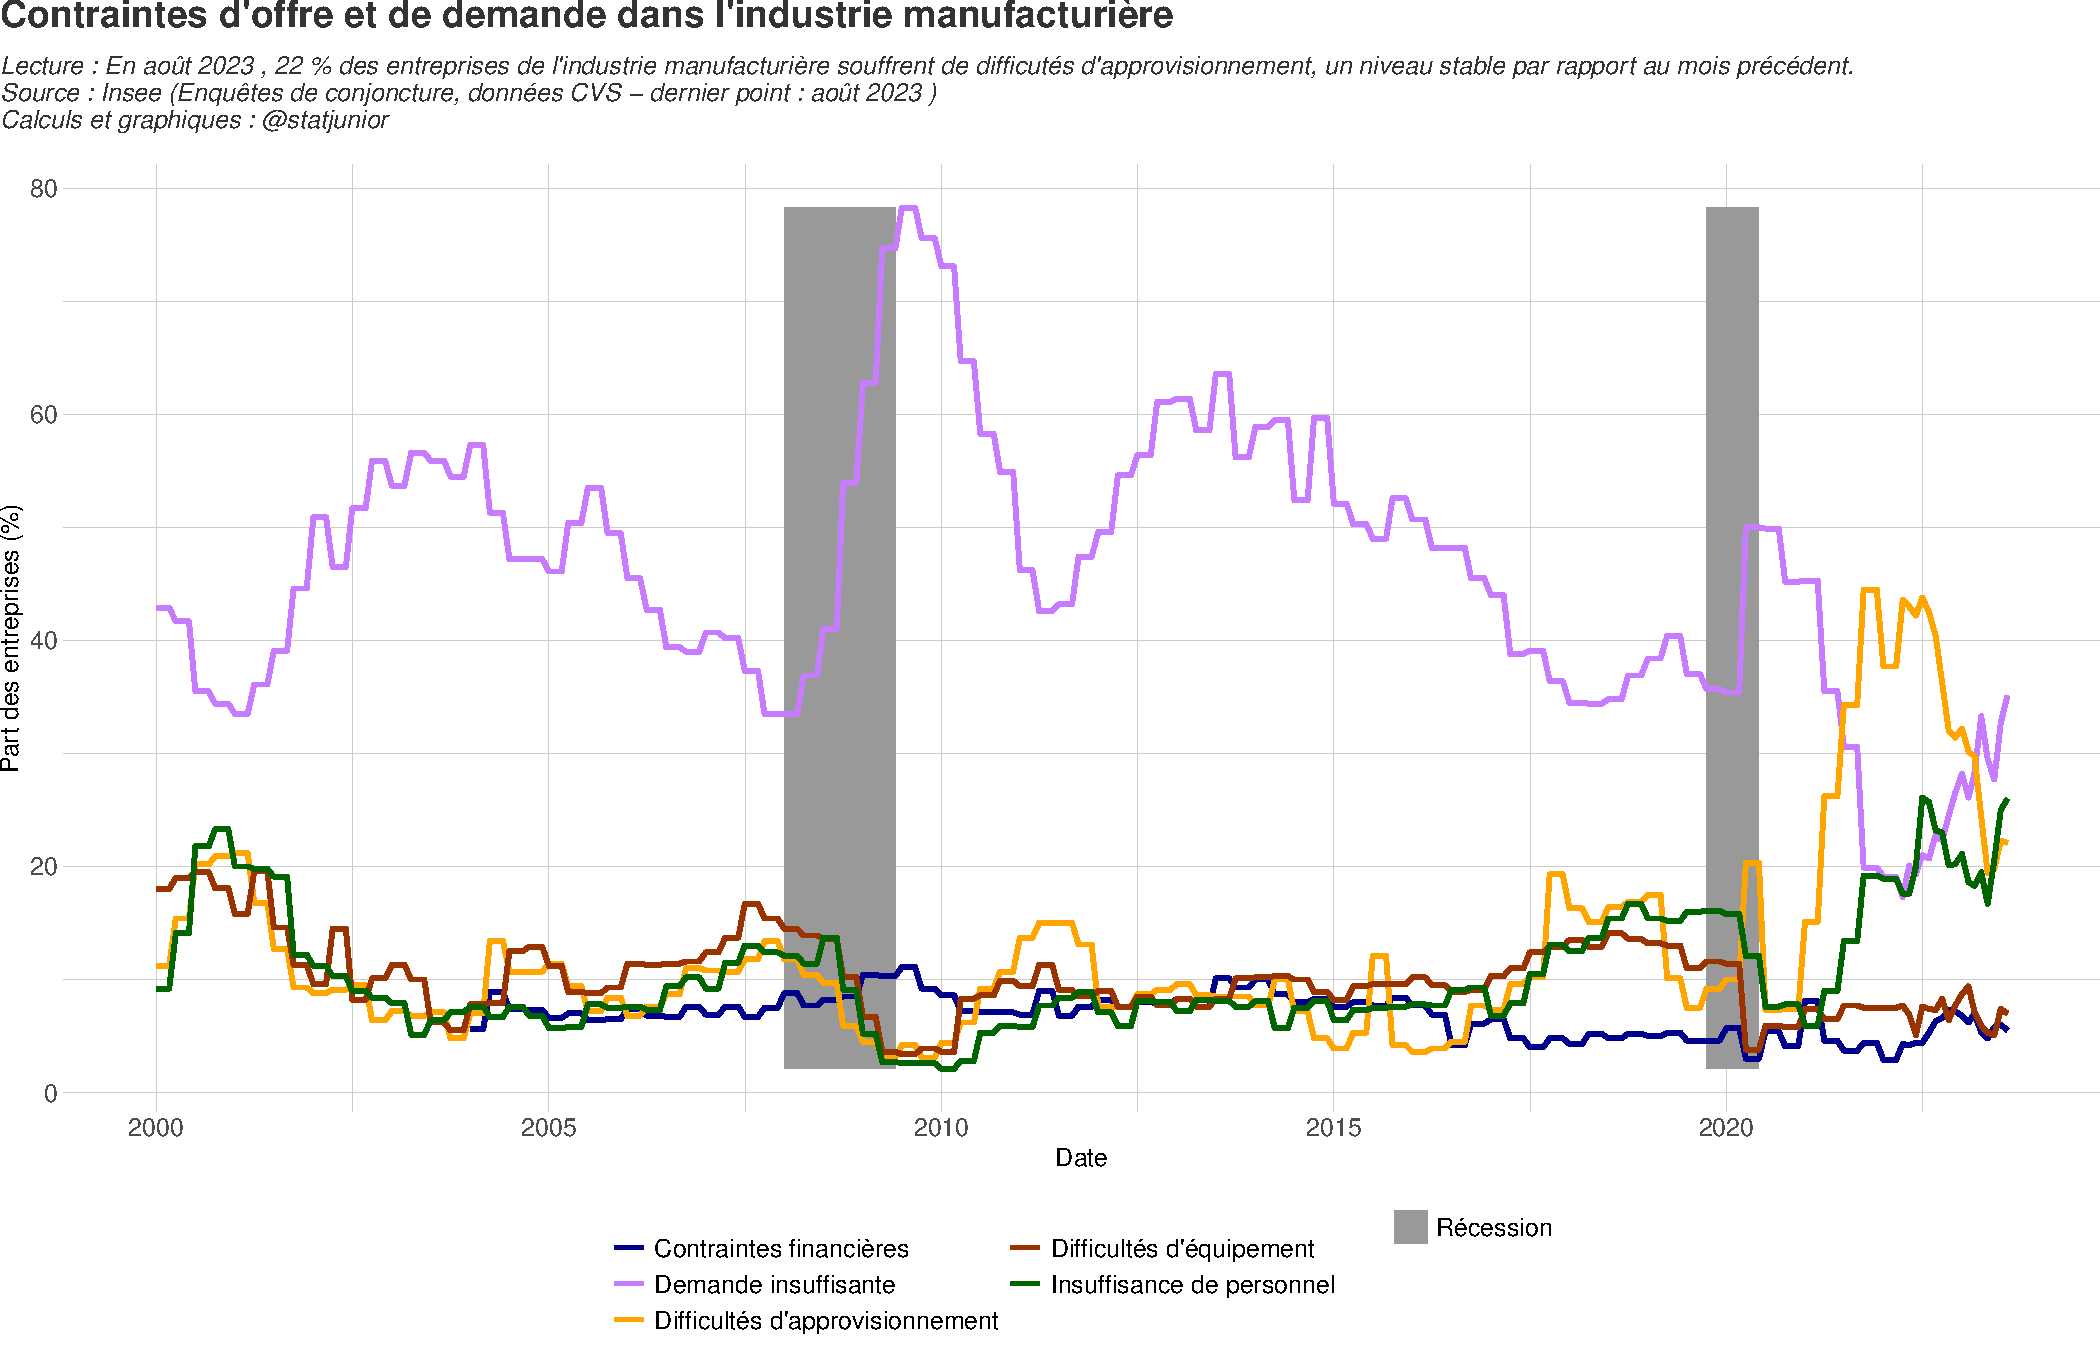
\includegraphics[keepaspectratio]{rapport_pdf_enquete_conj_files/figure-latex/unnamed-chunk-8-1.pdf}}

\end{document}
